\documentclass{standalone}
\usepackage{tikz}
\begin{document}
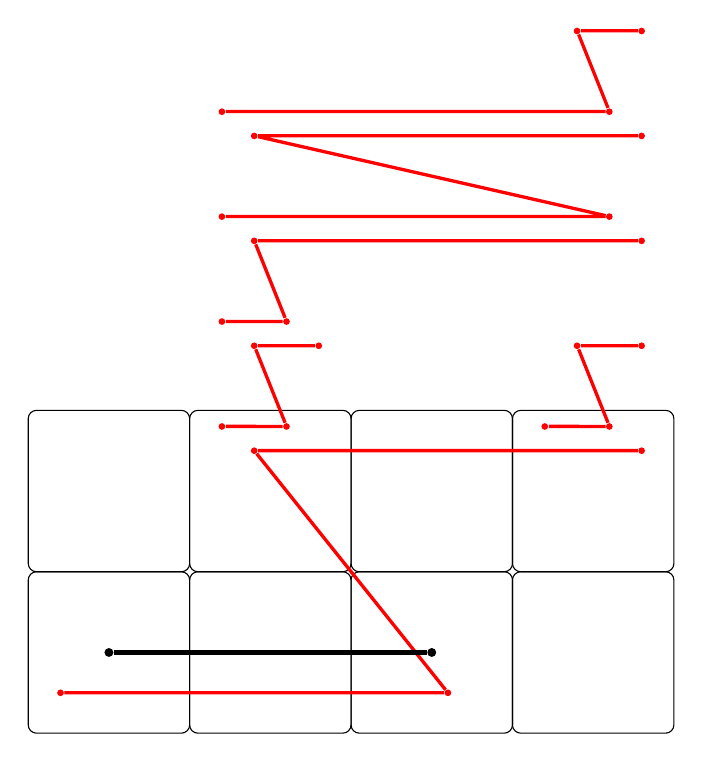
\begin{tikzpicture}[scale=2.05]
  % draw rounded cell boxes
  \draw[rounded corners=3pt] (0,0) rectangle (1,1);
  \draw[rounded corners=3pt] (0,1) rectangle (1,2);
  \draw[rounded corners=3pt] (1,0) rectangle (2,1);
  \draw[rounded corners=3pt] (1,1) rectangle (2,2);
  \draw[rounded corners=3pt] (2,0) rectangle (3,1);
  \draw[rounded corners=3pt] (2,1) rectangle (3,2);
  \draw[rounded corners=3pt] (3,0) rectangle (4,1);
  \draw[rounded corners=3pt] (3,1) rectangle (4,2);
  \node[circle, fill=red, inner sep=0.03cm] (obs4362281584_pt0) at (0.2,0.25) {};
  \node[circle, fill=red, inner sep=0.03cm] (obs4362281584_pt1) at (1.4,1.75) {};
  \node[circle, fill=red, inner sep=0.03cm] (obs4362281584_pt2) at (2.6,0.25) {};
  \node[circle, fill=red, inner sep=0.03cm] (obs4362281584_pt3) at (3.8,1.75) {};
  \draw[red, line width=1.2pt] (obs4362281584_pt0) -- (obs4362281584_pt2) -- (obs4362281584_pt1) -- (obs4362281584_pt3);
  \node[circle, fill=red, inner sep=0.03cm] (obs4362281632_pt0) at (1.2,1.9000000000000001) {};
  \node[circle, fill=red, inner sep=0.03cm] (obs4362281632_pt1) at (1.4,2.4000000000000004) {};
  \node[circle, fill=red, inner sep=0.03cm] (obs4362281632_pt2) at (1.6,1.9000000000000001) {};
  \node[circle, fill=red, inner sep=0.03cm] (obs4362281632_pt3) at (1.8,2.4000000000000004) {};
  \draw[red, line width=1.2pt] (obs4362281632_pt0) -- (obs4362281632_pt2) -- (obs4362281632_pt1) -- (obs4362281632_pt3);
  \node[circle, fill=red, inner sep=0.03cm] (obs4362281680_pt0) at (1.2,2.5500000000000003) {};
  \node[circle, fill=red, inner sep=0.03cm] (obs4362281680_pt1) at (1.4,3.0500000000000003) {};
  \node[circle, fill=red, inner sep=0.03cm] (obs4362281680_pt2) at (1.6,2.5500000000000003) {};
  \node[circle, fill=red, inner sep=0.03cm] (obs4362281680_pt3) at (3.8,3.0500000000000003) {};
  \draw[red, line width=1.2pt] (obs4362281680_pt0) -- (obs4362281680_pt2) -- (obs4362281680_pt1) -- (obs4362281680_pt3);
  \node[circle, fill=red, inner sep=0.03cm] (obs4362281728_pt0) at (1.2,3.200000000000001) {};
  \node[circle, fill=red, inner sep=0.03cm] (obs4362281728_pt1) at (1.4,3.700000000000001) {};
  \node[circle, fill=red, inner sep=0.03cm] (obs4362281728_pt2) at (3.6,3.200000000000001) {};
  \node[circle, fill=red, inner sep=0.03cm] (obs4362281728_pt3) at (3.8,3.700000000000001) {};
  \draw[red, line width=1.2pt] (obs4362281728_pt0) -- (obs4362281728_pt2) -- (obs4362281728_pt1) -- (obs4362281728_pt3);
  \node[circle, fill=red, inner sep=0.03cm] (obs4362281776_pt0) at (1.2,3.850000000000001) {};
  \node[circle, fill=red, inner sep=0.03cm] (obs4362281776_pt1) at (3.4,4.350000000000001) {};
  \node[circle, fill=red, inner sep=0.03cm] (obs4362281776_pt2) at (3.6,3.850000000000001) {};
  \node[circle, fill=red, inner sep=0.03cm] (obs4362281776_pt3) at (3.8,4.350000000000001) {};
  \draw[red, line width=1.2pt] (obs4362281776_pt0) -- (obs4362281776_pt2) -- (obs4362281776_pt1) -- (obs4362281776_pt3);
  \node[circle, fill=red, inner sep=0.03cm] (obs4362281824_pt0) at (3.2,1.9000000000000001) {};
  \node[circle, fill=red, inner sep=0.03cm] (obs4362281824_pt1) at (3.4,2.4000000000000004) {};
  \node[circle, fill=red, inner sep=0.03cm] (obs4362281824_pt2) at (3.6,1.9000000000000001) {};
  \node[circle, fill=red, inner sep=0.03cm] (obs4362281824_pt3) at (3.8,2.4000000000000004) {};
  \draw[red, line width=1.2pt] (obs4362281824_pt0) -- (obs4362281824_pt2) -- (obs4362281824_pt1) -- (obs4362281824_pt3);
  % draw black chords for chord_row_cells
  \node[circle, fill=black, inner sep=0.04cm] (chord_row0_left) at (0.5,0.5) {};
  \node[circle, fill=black, inner sep=0.04cm] (chord_row0_right) at (2.5,0.5) {};
  \draw[black, line width=1.5pt] (chord_row0_left) -- (chord_row0_right);
\end{tikzpicture}
\end{document}